\section{Vowel count}
\subsection{Aim}
To count the occurences of vowels in a string

\subsection{Code}
\begin{lstlisting}
  DATA SEGMENT
  str DB 'hello world', '$'
  strlen EQU $~str
  nvowels DW ?
DATA ENDS

CODE SEGMENT
ASSUME CS:CODE, DS:DATA
START:
  MOV AX, DATA
  MOV DS, AX
  MOV CX, strlen
  XOR BX, BX
  LEA SI, str

COMP:
  CMP BYTE PTR SI, 'a'
  JE INCR
  CMP BYTE PTR SI, 'e'
  JE INCR
  CMP BYTE PTR SI, 'i'
  JE INCR
  CMP BYTE PTR SI, 'o'
  JE INCR
  CMP BYTE PTR SI, 'u'
  JE INCR
  JMP INCRC
  
INCR:
  INC BX
  
INCRC:
  INC SI
  LOOP COMP
  
EXIT:
  MOV nvowels, BX
  MOV AH, 4CH
  INT 21H
CODE ENDS
END START
\end{lstlisting}

\subsection{Output}
\begin{center}
	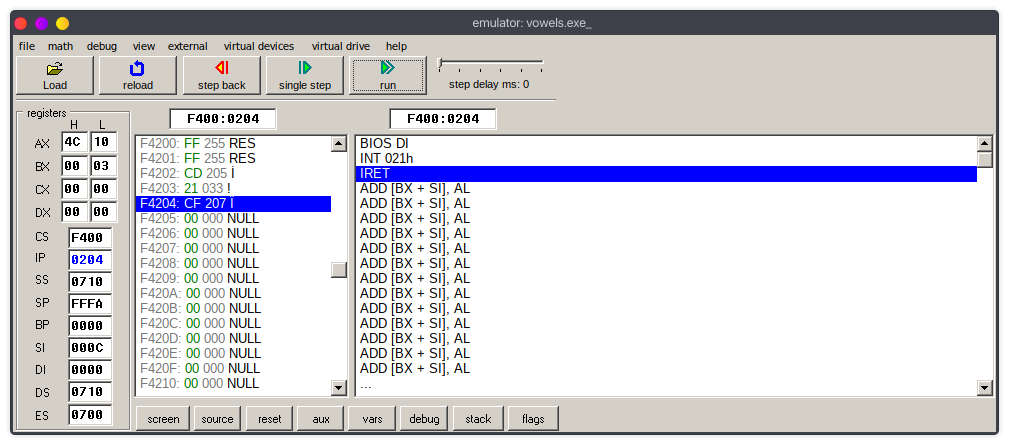
\includegraphics[width=0.90\textwidth]{img/p18/ss1.png}
	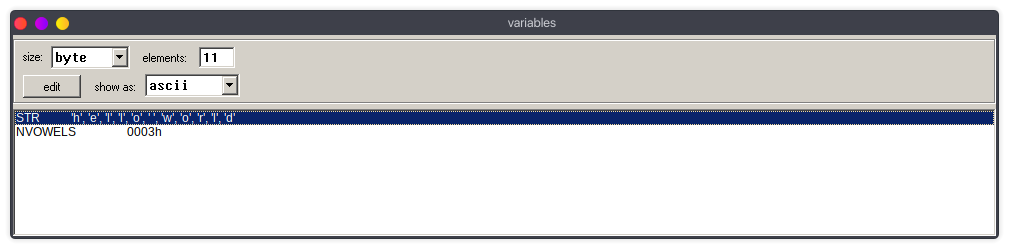
\includegraphics[width=0.90\textwidth]{img/p18/ss2.png}
\end{center}

\subsection{Result}
The number of vowels in a string was counted

